% =====================================================================
% SECCIÓN 5: RESULTADOS PRINCIPALES Y CONTRASTACIÓN FORMAL
% =====================================================================

% ---------------------------------------------------------------------
% Diapositiva 12: Protocolo y Métricas
% ---------------------------------------------------------------------
\section{Evaluación}

\begin{frame}{Protocolo de evaluación y métricas multidimensionales}
  \framesubtitle{Evaluación robusta ante desbalance y estimación de incertidumbre}

  \begin{columns}[T]
    \column{0.52\textwidth}
    \begin{itemize}
      \item \textbf{Métrica rectora ($F_1$-macro):} Media armónica no ponderada entre ambas clases; balancea control y depresión.
      \item \textbf{Sensibilidad clínica ($F_1$-depresión):} Rendimiento exclusivo sobre la clase positiva de interés.
      \item \textbf{Discriminación (AUC-ROC):} Capacidad probabilística independiente del umbral de corte.
      \item \textbf{Acuerdo por azar ($\kappa$ de Cohen):} Fiabilidad ajustada por la prevalencia de las clases.
    \end{itemize}

    \column{0.46\textwidth}
    \ugrblock{Incertidumbre por Bootstrap ($B=2\,000$)}{
      \begin{itemize}
        \item \textbf{Conglomerados por usuario:} Remuestreo en bloque de los 64 autores del test nativo común.
        \item \textbf{Independencia real:} Conserva intacta la estructura correlacionada de textos por autor.
        \item \textbf{Intervalos de confianza:} Método percentil empírico del 95\,\% ($[\alpha/2;\; 1 - \alpha/2]$).
      \end{itemize}
    }
  \end{columns}

  \note{
    Ante el desbalance de clases, seleccionamos F1-macro como métrica principal y AUC-ROC como métrica umbral-independiente. Para medir la variabilidad real, aplicamos un bootstrap de conglomerados de 2000 réplicas sobre los 64 usuarios del conjunto de prueba, respetando la correlación intra-sujeto.
  }
\end{frame}

% ---------------------------------------------------------------------
% Diapositiva 13: Resultados en el Test Nativo Común
% ---------------------------------------------------------------------
\begin{frame}{Resultados principales sobre el test nativo común}
  \framesubtitle{Evaluación sobre 250\,847 tweets de 64 usuarios independientes}

  \begin{table}
    \centering\scriptsize
    \setlength{\tabcolsep}{4pt}
    \caption{Métricas con intervalos de confianza del 95\,\% (Bootstrap de 64 usuarios, $B=2\,000$).}
    \begin{tabular}{lcccc}
      \toprule
      \textbf{Modelo evaluado} & \textbf{F1-macro} & \textbf{F1 depresión} & \textbf{AUC-ROC} & \textbf{Kappa ($\boldsymbol{\kappa}$)} \\
      \midrule
      LR TF-IDF (submuestreo) & 0{,}653 \tiny{[0{,}605; 0{,}691]} & 0{,}544 & 0{,}753 \tiny{[0{,}715; 0{,}788]} & 0{,}317 \\
      LR TF-IDF (ponderado) & 0{,}655 \tiny{[0{,}606; 0{,}693]} & 0{,}546 & 0{,}755 \tiny{[0{,}718; 0{,}790]} & 0{,}321 \\
      SVM lineal TF-IDF & 0{,}653 \tiny{[0{,}605; 0{,}692]} & 0{,}544 & 0{,}754 \tiny{[0{,}716; 0{,}787]} & 0{,}318 \\
      LR Combinado (19 rasgos) & 0{,}644 \tiny{[0{,}593; 0{,}684]} & 0{,}540 & 0{,}750 \tiny{[0{,}710; 0{,}785]} & 0{,}303 \\
      \rowcolor{filaResaltada}
      \textbf{BETO mono (contextual)} & \textbf{0{,}717} \tiny{[0{,}665; 0{,}759]} & \textbf{0{,}613} & \textbf{0{,}808} \tiny{[0{,}755; 0{,}849]} & \textbf{0{,}437} \\
      \bottomrule
    \end{tabular}
  \end{table}

  \vskip-0.15cm
  \begin{columns}[T]
    \column{0.49\textwidth}
    \ugrblockok{Superioridad de BETO}{
      BETO supera a la mejor línea base léxica en \textbf{+6{,}2 puntos de F1-macro} y \textbf{+5{,}2 puntos de AUC-ROC}.
    }
    \column{0.49\textwidth}
    \ugralert{Hallazgo sobre rasgos expertos}{
      Los 19 rasgos psicolingüísticos \textbf{no superaron} a los n-gramas puros (F1 0{,}644 vs.\ 0{,}655); el vocabulario absorbe la señal.
    }
  \end{columns}

  \note{
    En el conjunto nativo común, las líneas base clásicas convergen en 0.655 de F1-macro y 0.755 de AUC. Los rasgos psicolingüísticos no aportan ganancia frente al TF-IDF. Por su parte, BETO mono alcanza 0.717 de F1-macro y 0.808 de AUC, logrando una diferencia sustantiva superior a 6 puntos porcentuales.
  }
\end{frame}

% ---------------------------------------------------------------------
% Diapositiva 14: Discriminación y Curvas ROC
% ---------------------------------------------------------------------
\begin{frame}{Capacidad de discriminación y matriz de confusión}
  \framesubtitle{Análisis de curvas ROC y estructura de clasificación de BETO}

  \begin{columns}[T]
    \column{0.50\textwidth}
    \begin{center}
      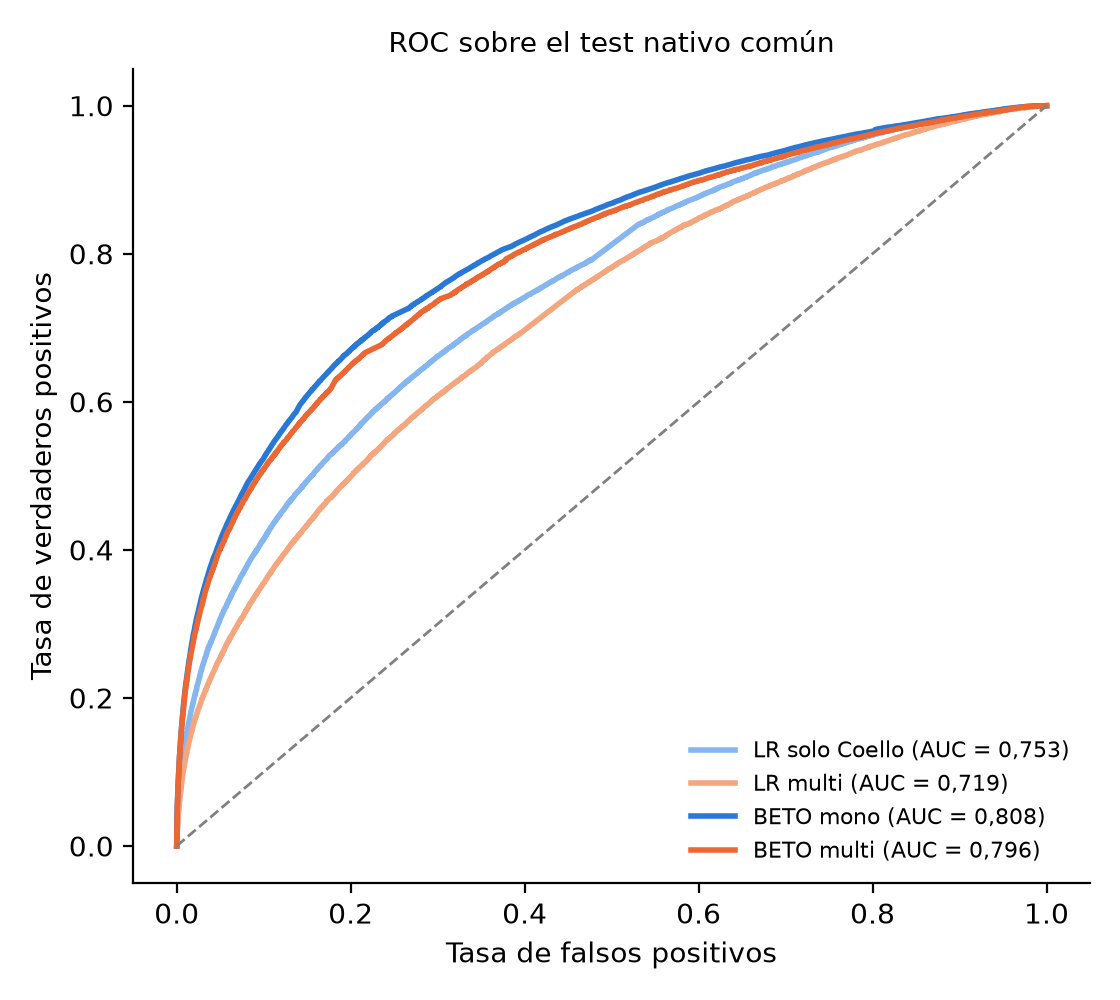
\includegraphics[width=\textwidth,height=0.48\textheight,keepaspectratio]{roc_test_nativo.png}
      \vskip-0.1cm
      {\tiny\color{ugrGris}Figura 2: Curvas ROC sobre el test nativo (BETO domina con AUC = 0{,}808).\par}
    \end{center}

    \column{0.50\textwidth}
    \begin{center}
      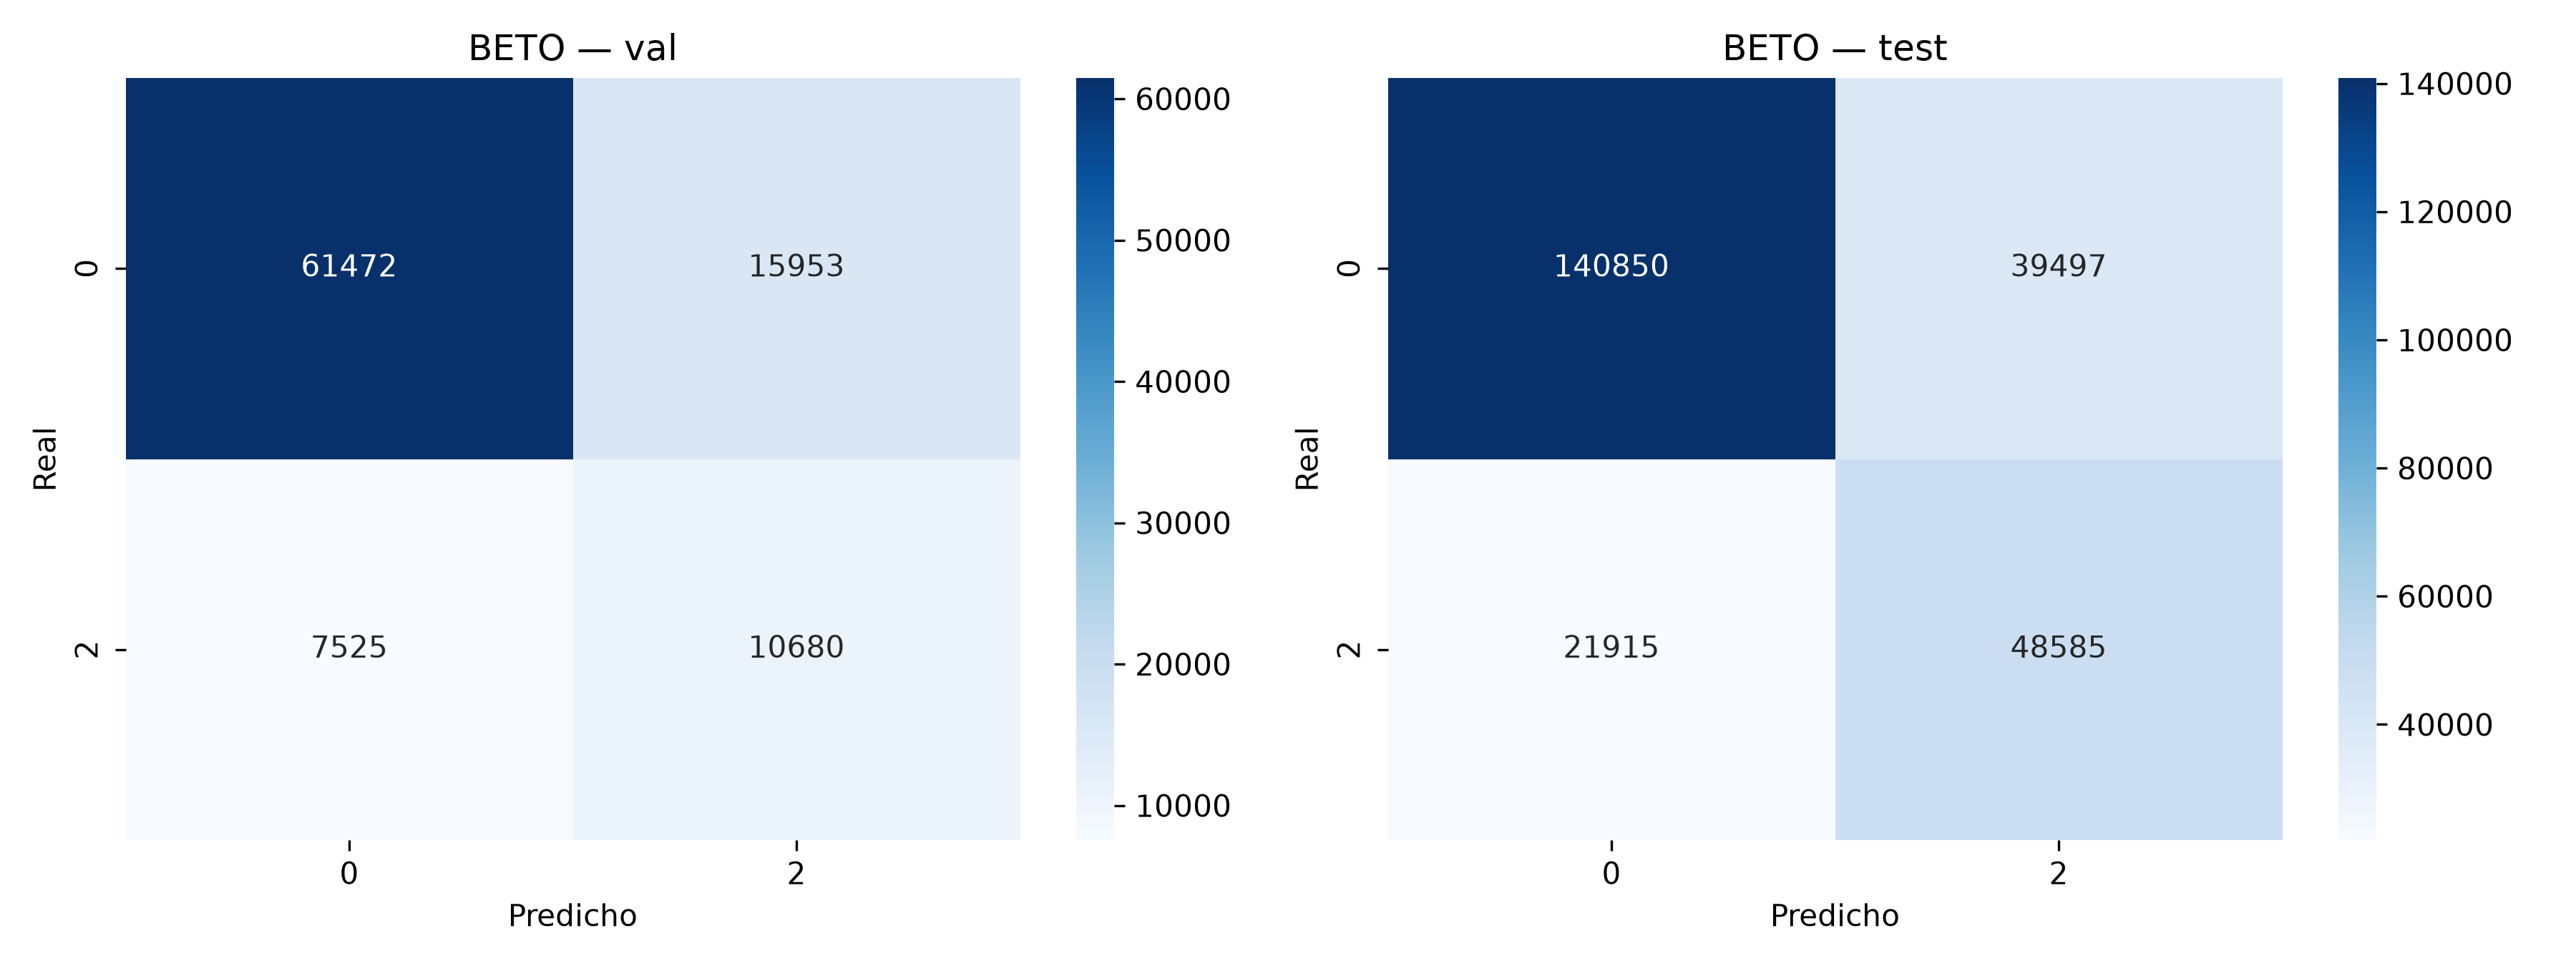
\includegraphics[width=\textwidth,height=0.48\textheight,keepaspectratio]{beto_confusion_matrix.png}
      \vskip-0.1cm
      {\tiny\color{ugrGris}Figura 3: Matriz de confusión normalizada de BETO mono (sensibilidad 69\,\%, especificidad 78\,\%).\par}
    \end{center}
  \end{columns}

  \vskip-0.1cm
  \begin{center}
    {\scriptsize\color{ugrAzul}\textbf{Compromiso clínico:} A nivel de publicación individual, la especificidad del 78\,\% minimiza falsas alarmas, mientras la agregación por perfil compensa falsos negativos.\par}
  \end{center}

  \note{
    La curva ROC de BETO domina de punta a punta a todas las líneas base. En la matriz de confusión observamos un equilibrio sólido: 78% de especificidad y 69% de sensibilidad sobre publicaciones aisladas. En cribado poblacional, este balance es óptimo para evitar saturar el sistema con falsos positivos.
  }
\end{frame}

% ---------------------------------------------------------------------
% Diapositiva 15: Contrastación Formal de Hipótesis
% ---------------------------------------------------------------------
\begin{frame}{Contrastación formal de la hipótesis ($H_1$ vs.\ $H_0$)}
  \framesubtitle{Diferencias pareadas directas e inferencia estadística conclusiva}

  \begin{table}
    \centering\scriptsize
    \setlength{\tabcolsep}{4pt}
    \caption{Diferencias pareadas ($\text{BETO} - \text{Línea Base}$) sobre las $2\,000$ réplicas de bootstrap.}
    \begin{tabular}{lcccc}
      \toprule
      \textbf{Comparación pareada} & $\boldsymbol{\Delta F_1}$\textbf{-macro} & $\boldsymbol{\Delta}$\textbf{AUC-ROC} & $\boldsymbol{\Delta\kappa}$ & $\boldsymbol{p}$\textbf{-valor empírico} \\
      \midrule
      BETO mono $-$ LR mono & \textbf{+0{,}062} \tiny{[0{,}038; 0{,}081]} & \textbf{+0{,}052} \tiny{[0{,}024; 0{,}077]} & \textbf{+0{,}116} \tiny{[0{,}068; 0{,}155]} & $p < 0{,}0005$ \\
      BETO mono $-$ SVM mono & \textbf{+0{,}063} \tiny{[0{,}040; 0{,}081]} & \textbf{+0{,}054} \tiny{[0{,}026; 0{,}077]} & \textbf{+0{,}119} \tiny{[0{,}072; 0{,}156]} & $p < 0{,}0005$ \\
      \bottomrule
    \end{tabular}
  \end{table}

  \vskip-0.1cm
  \ugrblockok{Decisión formal}{
    \begin{itemize}
      \item En el \textbf{100\,\% de las $2\,000$ réplicas} de remuestreo pareado por conglomerados de usuarios, BETO superó tanto a la Regresión Logística como a la SVM lineal.
      \item Los extremos inferiores del IC 95\,\% excluyen holgadamente el valor nulo ($\Delta F_1 > +0{,}038 > 0$).
      \item \textbf{Veredicto formal:} \textbf{Se rechaza $H_0$ y se acepta $H_1$} a nivel de publicación: BETO aporta una mejora predictiva estadísticamente demostrada y consistente.
    \end{itemize}
  }

  \note{
    La contrastación formal es contundente: réplica por réplica en el bootstrap pareado, BETO supera a las líneas base léxicas en el 100% de los casos. El extremo inferior del IC 95% para Delta F1-macro es de +0.038 y para Delta AUC de +0.024. Ambos son estrictamente mayores que cero. Se rechaza categóricamente H0 y se acepta H1.
  }
\end{frame}
